
%%%%%%%%%%%%%%%%%%%%%%% file typeinst.tex %%%%%%%%%%%%%%%%%%%%%%%%%
%
% This  is the LaTeX source for the instructions to authors using
% the LaTeX document class 'llncs.cls' for contributions to
% the Lecture Notes in Computer Sciences series.
% http://www.springer.com/lncs       Springer Heidelberg 2006/05/04
%
% It may be used as a template for your own input - copy it
% to a new file with a new name and use it as the basis
% for your article.
%
% NB: the document class 'llncs' has its own and detailed documentation, see
% ftp://ftp.springer.de/data/pubftp/pub/tex/latex/llncs/latex2e/llncsdoc.pdf
%
%%%%%%%%%%%%%%%%%%%%%%%%%%%%%%%%%%%%%%%%%%%%%%%%%%%%%%%%%%%%%%%%%%%


\documentclass[runningheads]{llncs}

\usepackage{amssymb}
\usepackage{cite}
\setcounter{tocdepth}{3}
\usepackage{graphicx}

\usepackage{url}
\urldef{\mailsa}\path|{alfred.hofmann,ursula.barth,ingrid.beyer,natalie.brecht,|
\urldef{\mailsb}\path|christine.guenther,frank.holzwarth,piamaria.karbach,|
\urldef{\mailsc}\path|anna.kramer,erika.siebert-cole,lncs}@springer.com|
\newcommand{\keywords}[1]{\par\addvspace\baselineskip
\noindent\keywordname\enspace\ignorespaces#1}

\newenvironment{myepigraph}
  {\par\hfill\itshape
   \begin{tabular}{@{}r@{}}} % 2em from the right margin
  {\end{tabular}\par\medskip}


\newcommand{\bi}{\begin{itemize}}
\newcommand{\ei}{\end{itemize}}
\newcommand{\be}{\begin{enumerate}}
\newcommand{\ee}{\end{enumerate}}

\newcommand{\fig}[1]{Figure~\ref{fig:#1}}
\newcommand{\eq}[1]{Equation~\ref{eq:#1}}
\newcommand{\tion}[1]{\S\ref{sec:#1}}


\usepackage[small,compact]{titlesec}



\usepackage{times}
\def\baselinestretch{0.95}


 \usepackage[font={small}]{caption, subfig}
 \renewcommand{\figurename}{Fig.}
 \renewcommand{\tablename}{Tab.}
\usepackage{enumitem}
\setlength{\abovecaptionskip}{1ex}
 \setlength{\belowcaptionskip}{1ex}
 \setlength{\floatsep}{1ex}
 \setlength{\textfloatsep}{1ex}
\setlist{nosep}

%\usepackage{biblatex}
%\renewcommand*{\bibfont}{\footnotesize}
%\usepackage[sort&compress]{natbib}  
 \newcommand{\bibfont}{\tiny}
% \setlength{\bibsep}{0ex}
%\renewcommand\section{\@startsection{section}{1}{\z@}{-10\p@ \@plus -4\p@ \@minus -4\p@}{5\p@ \@plus 4\p@ \@minus 4\p@}{\normalfont\large\bfseries\boldmath\rightskip=\z@ \@plus 8em\pretolerance=10000 }}


\begin{document}


\mainmatter  % start of an individual contribution

% first the title is needed
\title{Finding Explanations for Multi-Objective Optimization
(in Near-Linear Time)}

% a short form should be given in case it is too long for the running head
\titlerunning{SSBSE'15}

% the name(s) of the author(s) follow(s) next
%
% NB: Chinese authors should write their first names(s) in front of
% their surnames. This ensures that the names appear correctly in
% the running heads and the author index.
%
\author{Authors suppressed for blind review}

%<nalekkalapudi@mix.wvu.edu>Tim Menzies%
%%\and Ursula Barth\and Ingrid Beyer\and Natalie Brecht\and\\
%Christine G\"{u}nther\and Frank Holzwarth\and Pia Maria Karbach \and\\
%Anna Kramer\and Erika
%Siebert-Cole}
%
\authorrunning{Explaing MOEAs, SSBSE'15}
% (feature abused for this document to repeat the title also on left hand pages)

% the affiliations are given next; don't give your e-mail address
% unless you accept that it will be published
\institute{Institution suppressed for blind review}

%
% NB: a more complex sample for affiliations and the mapping to the
% corresponding authors can be found in the file "llncs.dem"
% (search for the string "\mainmatter" where a contribution starts).
% "llncs.dem" accompanies the document class "llncs.cls".
%
 
\maketitle


\begin{abstract}
CT0 is an algorithm for summarizing trade-offs in multi-objective problems.
From that summary, humans can read recommendations for their systems.
This paper evaluates those recommendations using data
generated from   (a) the POM3 model of agile selection
of tasks; (b) four COCOMO-suite predictors for software
development effort, months, defects and risk.

CT0 is a very fast algorithm- both theoretically and empirically.
For example, for the COCOMO-suite models, CT0 terminated
in 3 seconds while standard optimizers (NSGA-II and SPEA2)
took 150 seconds.
Further, the  generated 
explanations for CT0 were just as effective as from other optimizers.

Hence, we recommend CT0 when some succinct summary
has to be rapidly generated (e.g.  in some
interactive design meeting). CT0 could also be
useful as post-processor to other optimizers (to
generate succinct explanations of their conclusions)
or as a optimizer to other optimizers (by
constraining those other optimizers to only search
the regions recommended by CT0).

\keywords{Software engineering, explanation, optimization, multi-objective.}
\end{abstract}



\section{Introduction}

\begin{myepigraph}
``If you cannot- in the long run- tell  everyone what \\
 you have been doing, your  doing has been worthless.''\\
 {\em-- Erwin Schr\"odinger}

\end{myepigraph}


Explaining the results of
multi-objective optimization to a user
can be problematic.
A typical run of a multi-objective optimizer
can process thousands to millions of examples.
It is an overwhelming task for humans to
certify the correctness of conclusions generated
from so many results. Verrappa and Leiter warn that
\begin{quote}
``..for industrial problems, these algorithms generate
(many) solutions, which makes the tasks of
understanding them and selecting one among them
difficult and time consuming''~\cite{veer11}.
\end{quote}
Even if explanations are constrained to
 (say) just a few hundred examples taken from the Pareto
frontier, this can still confuse the user.
 Valerdi notes that it can take days for
panels of human experts to rigorously review even a few dozen
examples~\cite{valerdi11}.  
For example, once had a 
client who disputed the results of our  analysis.
They
demanded to  audit the reasoning but
 when we delivered the 
of candidate solutions on the Pareto frontier,
they were overwhelmed by
the amount of information.  Flustered,
the client discounted the  analysis
and rejected our conclusions. From this experience, we learned that
to better support decision making in SBSE, we must better explain
SBSE results.

Other researchers have recognized the importance
of explanation.
It is known to be a key factor in selecting algorithms.
For example, in the field of machine learning,
``each time one of our favorite 
approaches has been applied in industry, each time the
comprehensibility of the results, though ill-defined, has
been a decisive factor of choice over an approach by pure
statistical means, or by neural networks.''~\cite{ag98}.
Analogous terms to explainability  in that community 
are ``comprehensibility'',
``interpretability''~\cite{maimon05} or ``understandability''~\cite{allahyari:user-oriented}.

In spite of the importance attributed to the subject,
explanation has not been extensively investigated in the context of SBSE.
One of the few papers that does is that of 
 Veerappa and Lieter~\cite{veerappa11} who
clustered examples from the Pareto
frontier (examples generated from a goal graph representation of requirements
for London ambulance services). In this approach,
``instead of having to inspect a large
number of individual solutions, (users) can look at a
much smaller number of groups of related solutions,
and focus their attention on the important
characteristics of the group rather than the
particularities of their individual solutions''~\cite{veerappa11}. 

XXXX after creating. still errors in comparisons

While an innovative and insightful study, there
are three open issues with that method:  (a)~the complexity
of clustering; (b)~erroneous conclusions could be generated from the users 
inspection of the clusters; (c)~introduced by users
incorrectly evaluation the value of generated recommendations.
 Veerappa and Lieter did not evaluate the effects
of the recommendations that could be generated by users browsing their
clusters. 
Also, their method could suffer from scalability issues since it
a post-processor
to a clustering algorithm (clustering is a slow process  requiring
 say, $O(N^2)$ comparisons
for the greedy agglomerate clustering algorithm used in that paper~\cite{koc11b}).

Accordingly, in this paper, when:
\be
\item Cluster using a near-linear time algorithm;
\item Better define the process by which recommendations are generated
      from clusters;
\item The generated recommendations are tested by generating more
examples from the model {\em after} the recommendations are imposed
as extra constraints on the model inputs.
\ee

\section{A Motivating Example}
\subsection{Our Problem}
To motivate this work, we offer the real-world goal that sparked this work.

The Software Engineering Institute (SEI:
http://www.sei.cmu.edu/) at Carnegie Mellon
University is a centralized repository for
qualitative and quantitative data collected from
software development for the United States
government and Department of Defense. Developers
across the country looked to SEI for explanations of
what factors effect their project (these
explanations are used to manage their current
projects and well as propose methods on how to
better handle their future projects in a better
manner).  Also, large scale policy decisions about
information technology are made by the
U.S. government, partially in consultation with
researchers at the SEI.

It is standard for the
SEI to issues ``fact sheets'' explaining their
lessons learned as well as explaining their advise
on best practice. These explanations are short
reports (rarely more than both sides of one piece of
paper) which are intended to give busy managers
quick guidance for their projects.  In the case of
quantitative data, these explanations may
contain some 2D plot showing how one
objective  (e.g. defects) changes in
response to changes in one input variable
(e.g. lines of code).

The veracity of these simple plots
of SE data is questionable. Even
for single goal reasoning such as defect reduction,
there  can only be  poorly
characterized via one input variable.  Menzies et
al. compared learners building models with $N=1$
of $N>1$ input variables: the models that used more
than one input performed better~\cite{me07b}.

Further, there are many recent SE research publications that
propose multiple competing goals for SE models; e.g.
\bi
\item 
Build software
{\em faster} using {\em less} effort with {\em fewer} bugs~\cite{elrawas10};
\item
Return defect predictors that find {\em most} defects in the {\em smallest}
parts of the code~\cite{arisholm06}.
\ei
As we move from single goal to
multiple-goal reasoning, the value of
simplistic  plots to explain effects in SE projects becomes even more
questionable. The SBSE experience is that reasoning
and trading off between multiple goals is much more
complex that browsing effects related to a single
isolated goal.

Worse yet, given all the context variables that can
be used to describe different software projects, it
is hard to believe that any {\em one} report can
explain {\em all} the effects seen in all different
kinds of software projects. Numerous recent reports
in empirical SE offer the same {\em locality
effect}; i.e. models generated using {\em all}
available data perform differently, and often worse, than
those learned from specific subsets~\cite{posnet11,betta12,me12d,yang13,emse12}.

\subsection{Our Solution}

New results suggest a resolution to the above
problems.  Firstly, work on {\em low dimensional
  approximations} of SE data shows we do not
need to reason about all the context variables
(since many are redundant or noisy). When applied to
SBSE, low dimensional approximations can
guide mutation strategies to find
better solutions one to two orders of magnitude
faster than standard evolutionary
optimizers~\cite{krall14,krall14b}.

Secondly, work on MOEA/D (multi-objective
evolutionary algorithms with decomposition~\cite{zhang07:TEC}) has
shown the benefits of dividing  problems into multiple cells, then 
optimizing each cell separately.  Note
that this approach is analogous (and actually
pre-dates) the locality work mentioned above.

The rest of this paper reports an experiment where we generate explanations
of the forces that impact a software project by combining
{\em decomposition} with {\em low dimensional approximations}. Our
system is called WICKED and has six parts:
\begin{itemize}
\item[W:]
\underline{{\bf W}}HERE is Menzies'  near-linear time clustering algorithms~\cite{me12d}  that uses lower dimensional approximations
to
decompose
data from models of SE processes into many small clusters,
\item [I:] \underline{{\bf I}}NFOGAIN~\cite{FayIra93Multi} 
finds what numeric ranges best predict for the different clusters.
\item[C:] To find rules that distinguish the clusters,
we apply Brieman's \underline{{\bf C}}ART,
algorithm~\cite{breiman84} to the data simplified by INFOGAIN.
\item[K:]
\underline{{\bf K}}ILL  prunes spurious leaf
branches generated by CART, thus shrinking the tree.
KILL outputs branches (conjunctions of {\em attribute=value} pairs)
that lead to clusters $C_0,C_1,C_2,..$.
\item[E:]
\underline{{\bf E}}NVY looks at  all clusters $C_i$ trying to find a nearby cluster $C_j$  
with better objective scores.
\item[D:] \underline{{\bf D}}ELTA is a contrast-set
  learner that reports the difference branches
  ending at $C_i$ and $C_j$.  \ei It is reasonable
  to ask why these six particular parts, and not six
  other.  All the above are motivated by the need
  for generation explanations, and keeping those
  explanations succinct.  Kelly's Personnel
  construct theory~\cite{kelly55} conjectures that
  humans do not explain of the world by studying all
  factors: rather, they find differences between
  things. ENVY and DELTA are our method of
  implementing Kelly's insight.

As to the other parts of WICKED, WHERE's
dimensionality reduction lets us ignore spurious
dimensions while we group the data. Once WHERE
terminates, then the only ranges that are
interesting are those that distinguish between the
clusters (and these are found by INFOGAIN).
INFOGAIN is a pre-processor to decision tree
learning and KILL is a post-processor.  The
combination of these pre-post-processors means that
the trees found by CART are very small. This, in
turn, means that the contrast found by ENVY+DELTA
are very succinct.

The output of WICKED is {\em recommendation} for
how we would improve all the examples in $C_i$. Expressed in terms
of evolutionary algorithms, {\em recommendation = mutation}; i.e. they
are the
suggestion on how to change examples in order to optimize
multiple objectives.
Return now to writing fact sheets from the SEI, we note that:
\bi
\item
INFOGAIN+CART+KILL generates very small trees (10 to 20 lines);
\item
ENVY and DELTA are very simple algorithms
that can be applied by humans while manually browsing CT0's trees;
\item
The experiments shown below demonstrate that DELTA's recommendation are just as effective
as the mutations proposed by standard 
optimizers 
(NSGA-II~\cite{deb00a} and SPEA2~cite{zit02}) for adjusting a
population in order to improve multiple objectives.
\item
All of WICKED's sub-routines
are  near-linear time algorithms
that terminate 100 times faster than standard optimizers.
\ei
Hence, we propose a modification to SEI's fact sheet:
they should old the trees
generated by WHERE+INFOGAIN+CART+KILL. From these, 
business users can apply ENVY+DELTA in order to
explore for themselves the effects in SEI's data.


{\scriptsize
\begin{alltt}
if cplx \(\le\) 1.1:                          Effort  Months   Defect Risk
.. if resl \(\le\) 3.2:
.. .. if pvol \(\le\) 1.1:
.. .. .. if site \(\le\) 1.0:
.. .. .. ..  then: ['__25']  #                 ?      ?        ?      ?
.. .. .. ..  else: ['__20']  #          d      ?      ?        ?      ?
.. .. if rely \(\le\) 1.0:
.. .. .. if pcap \(\le\) 0.9:
.. .. .. .. if ltex \(\le\) 1.0:
.. .. .. .. .. if site \(\le\) 1.0:
.. .. .. .. .. ..  then: ['__3']  #     a     ?        ?      ?       ?
.. .. .. .. .. ..  else: ['__1']  #     c     ?        ?      ?       ?
.. .. .. .. .. else: ['__6']  #        b      ?        ?      ?       ?
.. .. .. .. if ltex \(\le\) 1.0:
.. .. .. .. .. if pmat \(\le\) 3.9:
.. .. .. .. .. ..  then: ['__15']  #         ?        ?      ?       ?
.. .. .. .. .. else: ['__15']  #       e     ?        ?      ?       ?
\end{alltt}}
%cplx resl pvol site reply pcal ltex pmat




\section{Models}
pom

cocomo


\section{Code}
This section describes WHERE+CART+ENVY+DELTA.

\subsection{WHERE}
WHERE inputs a set of $N$ examples, each of which is a set of decisions $D$
mapped to a set of objectives  $O$, so $N_i= (D,O)$ (and usually $D>1$ and $O>1$ and 
$O<D$).
WHERE clusters the examples on the decisions and reports the average objective
scores for each objective in each cluster.

WHERE uses a dimensionality reduction heuristic proposed by
Faloutsos and Lin~\cite{Faloutsos1995}. The method 
inputs
$N$
examples $N_1,N_2,..$. Next, WHERE
picks any
point $N_i$ at random. Thirdly, WHERE
finds the point  {\em West}~$\in N$ that is
furthest\footnote{
 For this work, we use the standard Euclidean measure recommended for
instance-based reasoning by Aha et al.~\cite{aha91};
i.e. $\sqrt{\sum_i(x_i-y_i)^2}$ where $x_i,y_i$ 
are values normalized 0..1 for the range min..max.}
from $N_i$.
Finally, WHERE
finds the point {\em East}~$\in N$
that is furthest from {\em West} (and 
$c=\mathit{dist}(\mathit{West},\mathit{East})$).

To recursively cluster the data, WHERE iterates over $N_i \in N$
to find
\mbox{$a=\mathit{dist}(N_i,\mathit{West})$},
\mbox{$b=\mathit{dist}(N_i,\mathit{East})$},
\mbox{$x=(a^2 + c^2 - b^2)/(2c)$}.
This  $x$ value is the projection of $N_i$
on the line  running  {\em East} to {\em West}.  WHERE divides
the examples on the median $x$ value,
then recurses on each half. 
Recursion on
$N$ initial
examples stops when a sub-region
contains less that  $M$ examples (e.g. 
$M=\sqrt{N}$).

Note that this four-step  
process requires only $2N$ distance comparisons
per level of recursion and one call to a sorting routine
to find the median value. 
The total time for WHERE is some linear multiple of the sorting time
used to find the median at each level.
Assuming sorting takes time $O(NlogN)$, then we can say 
that WHERE runs in near linear time
(and not the $O(N^2)$ required for 
other clustering algorithms such as K-Means~\cite{hamerly2010making}).

\subsection{CART}

\subsection{ENVY}

\subsection{DELTA}


\section{Results}


The following results come  from a standard Python 2.7 interpreter
(not PyPy) running on a 2.6 GHz Mac Os/X with 4 GB of ram.
For NSGA-II,
we used the out-of-the-box version from DEAP, https://github.com/DEAP/deap.


In the following, we compared WICKED's results with
that of NSGA-II~\cite{deb00}.  NSGA-II is a genetic
algorithm (GA) with a highly optimized {\em select}
operator: \bi
\item Each generation builds generation $G+1$ by {\em selecting} better
individuals, {\em combining} some of their parts, then 
{\em mutating} the results 
(a little).
\item NSGA-II is a GA whose {\em select} operator 
uses a non-dominating sort
procedure to divide the solutions into {\em bands}
where {\em band}$_i$ dominates all of the solutions
in {\em band}$_{j>i}$ (and NSGA-II favors the
least-crowded solutions in the better bands).
\ei
One reason to favor NSGA-II as our comparison optimizer is 
 {\em repeatability}. 
Many multi-objective optimizers as MOEA/D~\cite{zhang07} 
and PSO~\cite{Poli07particleswarm}
are really {\em frameworks} within 
which an engineer has free reign to make numerous decisions
(evidence: review papers list dozens of variants on  PSO and MOEA/D ~\cite{V.Sedenka2010,5601760}).
Hence, in terms of {\em repeatability}, it can better to use precisely defined algorithms like NSGA-II.

Other reasons to use NSGA-II are that (a)~it is very widely used 
and (b)~there is no clear
consensus that some other algorithm is better.
When selecting a comparison algorithm,
we reached out to our SBSE colleagues to
find
which algorithms are accepted as ``best''.  However, no consensus was found.
On the other hand, it can be shown that NSGA-II is widely used.
In 2013, Sayyad and Ammar~\cite{sayyad13c} surveyed 36 SBSE papers where $\frac{21}{36}$
used NSGA-II  (of the others, 4 used some home-brew genetic algorithm and the remainder
each used some MOEA not used by any other paper).


\subsection{Runtimes}

Standard MOEAs require at least $N^2$ comparisons
between $N$ candidates, for each generation $G$ of the evolution. In theory,
WICKED is much faster than that:
\bi
\item The current implementation of WICKED uses $G=1$
since its recommendations are the results of one analysis of the data
(in future work, we plan to explore an iterative evolutionary version of the 
algorithm).
\item All the sub-routines of WICKED take near linear-time (the
slowest is CART that must sort all examples at each level of its trees).
\ei
On experimentation, WICKED's runtimes are consistent with its
theoretical properties. \fig{pomtimes} show the effect on runtimes
of increasing the initial population size for WICKED and NSGA-II.
The solid lines denote WICKED's performance: note that they are always less
that those seen with NSGA-II. 
The effect that WICKED runs faster than standard optimizers, is most
pronounced in the more complex models. In the POM3 results, some of the POM3 variants
take 100s of seconds to terminate. The same problems are handled by WICKER in
under one minute. 


% XXXnaveen
% for the runtime figures
% change CT to WICKED
% add space after label some xomo gr not xomogr
% delete all and delete os (so only 3 lines per optimizer)
% 2) any explnation for the spike in nsga at P=400?
% 3) are these repeats over 20 runs?
% 4) please confirm. popSize=200?

\begin{figure}
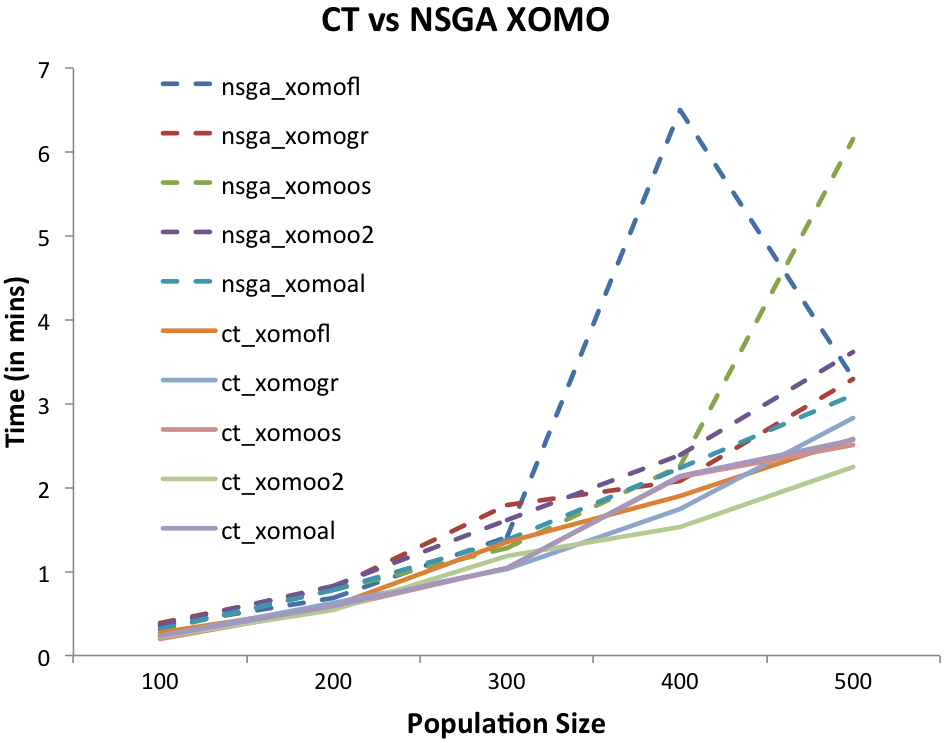
\includegraphics[width=6cm]{naveen/figures/xomotimes.png}
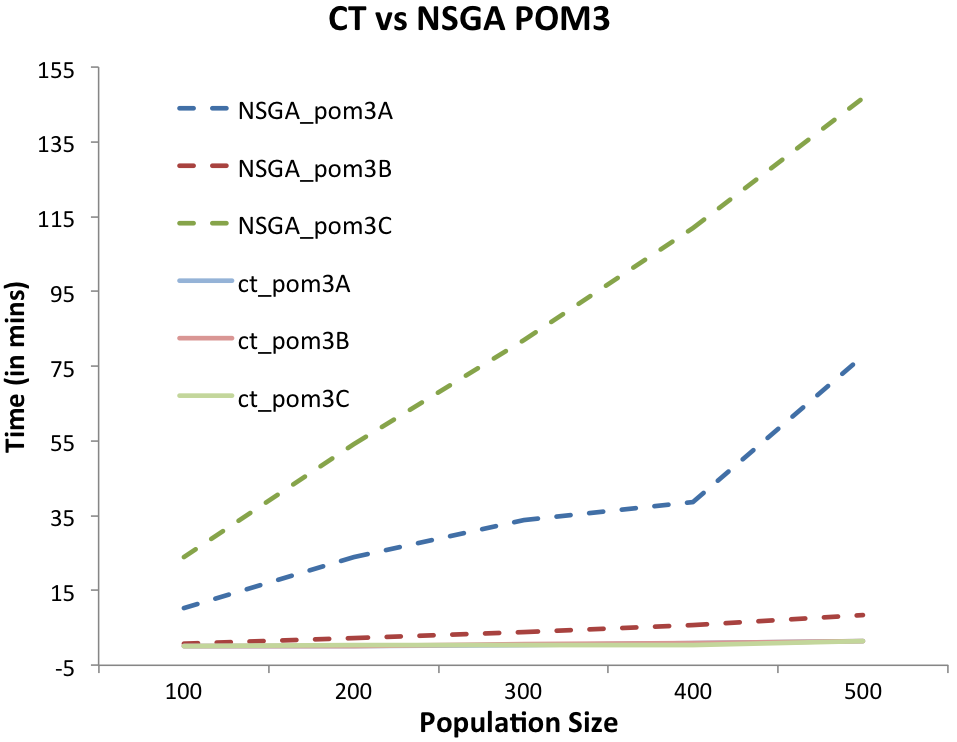
\includegraphics[width=6cm]{naveen/figures/pomtimes.png}
\caption{ Runtimes (minutes) for CT and NSGA II on POM Model
(means over 20 repeats)}\label{fig:pomtimes}
\end{figure}

Note that these runtime results come from an optimized version of WICKED.
Experiments are on-going with the Python profiler 
(to remove runtime bottlenecks). While those initial results are promising, we have
nothing definitive to report at this time.

\subsection{Optimization Improvements}

To explore optimization improvements, we:
\be
\item
Collected
{\em baseline}  distributions seen in the objectives of the initial population
(of 25 randomly generated individuals). 
\item Using the baseline as generation $G=1$, run NSGA-II until
no improvement in any objective for three generations;
\item Using that baseline, run WICKED once. For each cluster:
\bi
\item
Access the cluster items and the recommendation from the cluster;
\item
Re-run the model that generated the data using constraints
generated from that cluster; 
 \ei
\item Collected {\em treated} distributions from the output
of steps two and three.
\ee

\fig{optresults} shows the {\em baseline} and {\em treated} distributions
for:
\bi
\item For all the objectives of:
\bi
\item The three variants of POM3 shown in \fig{POM3abcd};
\item The three variants of XOMO shown in \fig{xomocases};
\ei
\ei
That figure presents displays results from 20
repeated runs as horizontal quartile charts. In that
figure, black dots denote median values and
horizontal lines denote the 25 to 75th percentile
range.  To simplify readability, for each objective,
all results and normalized 0..100 for the min to max
values seen for that objective.  Our three
treatments are shown in the ``Rx'' column: ``0''
denotes the baseline; ``W'' denotes WICKED, and
``N'' denotes NSGA-II.

In all these results, {\em lower} values are {\em
better} (exception: the {\em completion} goal in
POM3 which we seek to {\em maximize}). 

\renewcommand{\baselinestretch}{0.4}
\begin{figure}[!t]
\scriptsize
%\bf
\begin{minipage}{.52\linewidth}


\begin{tabular}{|l@{~}c@{~}c@{~}r|}
\arrayrulecolor{lightgray}
\rowcolor[gray]{.85} Fl     & Rx  & median &  \\ 
\rowcolor[gray]{1.0} effort  & 0 & 19 &  \quart{8.0}{15.0}{19.0} \\ 
 & W & 4 & \quart{0.0}{5.0}{4.0} \\ 
 & N & 11 &  \quart{4.0}{12.0}{11.0} \\ 
\hline\rowcolor[gray]{1.0} months  & 0 & 27 &  \quart{20.0}{1.0}{27.0} \\ 
 & W & 19 & \quart{15.0}{0.0}{19.0} \\ 
 & N & 36 &  \quart{27.0}{13.0}{36.0} \\ 
\hline\rowcolor[gray]{1.0} defects  & 0 & 22 &  \quart{10.0}{29.0}{22.0} \\ 
 & W & 2 & \quart{0.0}{3.0}{2.0} \\ 
 & N & 5 &  \quart{1.0}{7.0}{5.0} \\ 
\hline\rowcolor[gray]{1.0} risks  & 0 & 87 &  \quart{82.0}{5.0}{87.0} \\ 
 & W & 2 &  \quart{0.0}{0.0}{2.0} \\ 
 & N & 6 &  \quart{1.0}{9.0}{6.0} \\ 
\end{tabular}



\begin{tabular}{|l@{~}c@{~}c@{~}r|}
\arrayrulecolor{lightgray}
\rowcolor[gray]{.85}  GR  &Rx & median  &  \\ 
\rowcolor[gray]{1.0} effort  
 & 0 & 7 & \quart{3.0}{5.0}{7.0} \\ 
 & W & 3 &  \quart{0.0}{3.0}{3.0} \\ 
 & N & 13 &  \quart{6.0}{14.0}{13.0} \\ 
\hline\rowcolor[gray]{1.0} months  
 & 0 & 21 & \quart{17.0}{0.0}{21.0} \\ 
 & W & 23 &  \quart{18.0}{2.0}{23.0} \\ 
 & N & 39 &  \quart{29.0}{16.0}{39.0} \\ 
\hline\rowcolor[gray]{1.0} defects  
 & 0 & 16 &  \quart{7.0}{22.0}{16.0} \\ 
 & W & 1 &  \quart{0.0}{2.0}{1.0} \\ 
 & N & 4 &  \quart{1.0}{5.0}{4.0} \\ 
\hline\rowcolor[gray]{1.0} risks  
 & 0 & 74 &  \quart{66.0}{13.0}{74.0} \\ 
 & W & 6 &  \quart{3.0}{3.0}{6.0} \\ 
 & N & 5 &  \quart{0.0}{8.0}{5.0} \\ 
\end{tabular}



\begin{tabular}{|l@{~}c@{~}c@{~}r|}
\arrayrulecolor{lightgray}
\rowcolor[gray]{.85}02  & Rx & median  &  \\ 
\rowcolor[gray]{1.0} effort  & 0 & 5 &  \quart{3.0}{0.0}{5.0} \\ 
 & W & 7 &  \quart{6.0}{1.0}{7.0} \\ 
 & N & 13 &  \quart{6.0}{14.0}{13.0} \\ 
\hline\rowcolor[gray]{1.0} months  & 0 & 25 &  \quart{23.0}{0.0}{25.0} \\ 
 & W & 20 &  \quart{19.0}{0.0}{20.0} \\ 
 & N & 43 &  \quart{33.0}{20.0}{43.0} \\ 
\hline\rowcolor[gray]{1.0} defects  & 0 & 37 &  \quart{25.0}{24.0}{37.0} \\ 
 & W & 1 &  \quart{1.0}{0.0}{1.0} \\ 
 & N & 5 &  \quart{1.0}{8.0}{5.0} \\ 
\hline\rowcolor[gray]{1.0} risks  & 0 & 79 &  \quart{67.0}{16.0}{79.0} \\ 
 & W & 13 &  \quart{12.0}{0.0}{13.0} \\ 
 & N & 6 &  \quart{0.0}{10.0}{6.0} \\\hline 
\end{tabular}
\end{minipage}\begin{minipage}{.4\linewidth}

\begin{tabular}{|l@{~}c@{~}c@{~}r|}

\arrayrulecolor{lightgray}
\rowcolor[gray]{.85} POM3a  & Rx  & median & \\ 
\rowcolor[gray]{1.0} cost  & 0 & 32  & \quart{19.0}{28.0}{32.0} \\ 
 & W & 35 &  \quart{23.0}{25.0}{35.0} \\ 
 & N & 3 & \quart{3.0}{0.0}{3.0} \\ 
\hline\rowcolor[gray]{1.0} completion  & 0 & 85 &  \quart{74.0}{2.0}{85.0} \\ 
 & W & 75 &  \quart{65.0}{0.0}{75.0} \\ 
 & N & 86 &  \quart{78.0}{1.0}{86.0} \\ 
\hline\rowcolor[gray]{1.0} idle  & 0 & 22 & \quart{1.0}{36.0}{22.0} \\ 
 & W & 17 &  \quart{0.0}{29.0}{17.0} \\ 
 & N & 31 &  \quart{4.0}{45.0}{31.0} \\ 
\end{tabular}


\begin{tabular}{|l@{~}c@{~}c@{~}r|}
\arrayrulecolor{lightgray}
\rowcolor[gray]{.85} POM3B  & Rx & median &  \\ 
\rowcolor[gray]{1.0} cost  & 0 & 32 &  \quart{20.0}{27.0}{32.0} \\ 
 & W & 19 &  \quart{12.0}{14.0}{19.0} \\ 
 & N & 6 &  \quart{5.0}{0.0}{6.0} \\ 
\hline\rowcolor[gray]{1.0} completion  & 0 & 84 &  \quart{74.0}{2.0}{84.0} \\ 
 & W & 55 &  \quart{47.0}{0.0}{55.0} \\ 
 & N & 86 &  \quart{77.0}{2.0}{86.0} \\ 
\hline\rowcolor[gray]{1.0} idle  & 0 & 29 &  \quart{5.0}{37.0}{29.0} \\ 
 & W & 17 &  \quart{0.0}{27.0}{17.0} \\ 
 & N & 32 &  \quart{6.0}{47.0}{32.0} \\ 
\end{tabular}





\begin{tabular}{|l@{~}c@{~}c@{~}r|}
\arrayrulecolor{lightgray}
\rowcolor[gray]{.85} POM3C    & Rx & median & \\ 
\rowcolor[gray]{1.0} cost  & 0 & 40 &  \quart{27.0}{25.0}{40.0} \\ 
 & W & 31 &  \quart{20.0}{20.0}{31.0} \\ 
 & N & 10 &  \quart{8.0}{0.0}{10.0} \\ 
\hline\rowcolor[gray]{1.0} completion  & 0 & 90 &  \quart{82.0}{0.0}{90.0} \\ 
 & W & 63 & \quart{54.0}{1.0}{63.0} \\ 
 & N & 90 &  \quart{83.0}{1.0}{90.0} \\ 
\hline\rowcolor[gray]{1.0} idle  & 0 & 34 &  \quart{8.0}{33.0}{34.0} \\ 
 & W & 21 &  \quart{0.0}{25.0}{21.0} \\ 
 & N & 36 &  \quart{8.0}{41.0}{36.0} \\\hline
\end{tabular}~\\\vspace{2.11cm}~\\\end{minipage}

\caption{  XOMO results (left); POM3 results (right);
all results from 20 runs with different random seeds.
Big black dots show median values. 
Horizontal
lines show 25th to 75th percentile.
All results are normalized 0..100, min..max. 
Except for POM3's {\em completion} objective, 
{\em smaller} values are
{\em better}. In the ``Rx'' column,
``0,W,N'' denotes 
results from baseline,
WICKED, and  NSGA-II (respectively).
}\label{optresults}
\end{figure}
\renewcommand{\baselinestretch}{1}



\section{Explaining ``Explanation''}
As a starting point in this exploration of explanation,
it is important to distinguish between the
(1)~problem of explaining the output of an
multi-objective optimizer (discussed in this paper);
from the more complex problem of (2)~explaining how
that output was generated.  To put that another way:
we seek to explain eggs, but not
the chicken.

Next, a definition of  ``explanation'' is required such that:
\be
\item An explanation system can be designed;
\item It is possible to distinguish a  ``good'' for a ``bad'' explanation.
\ee
In the SE literature,
the general consensus in
software engineering is that ``good'' explanations
are succinct explanations~\cite{ag98,dej13z,fenton99}.
On this score, MOEAs fare poorly since their output can be very verbose
(hundreds or more examples from the Pareto frontier).


Also, cognitive science theory argues that
there is more to ``explaining'' something that just
showing it succinctly. According to Kelly's personal
construct theory (PCT) humans explain things via
``constructs'' that distinguish sets of examples~\cite{kelly55}.
So, for Kelly, human explanations are not about
``things'' in isolation but rather the {\em
differences between groups of things}. In data mining, finding
differences between things is called {\em contrast set learning}~\cite{webb09}.



Other  cognitive science research studied the activities
humans do during explanation generation.
Leake~\cite{leake91}
lists a dozen different tasks that humans perform when 
``explaining'' some phenomena. Leake does not claim
that the following list is complete; just that
it demonstrates  a wide range of
goal-based purposes for explanation, including:
\be
\item
Connect event to expected/believed conditions.
\item
Connect event to previously unexpected conditions.
\item
Find predictors for anomalous situation.
\item
Find repair points for causes of an undesirable state.
\item
Clarify current situation to predict effects or choose response.
\item
Find controllable (blockable or achievable) causes.
\item
Find actors’ contributions to outcome.
\item
Find motivations for anomalous actions or decisions.
\item
Find a within-theory derivation.
\ee
That is, to Leake, explanation is akin to planning
where the ``explainer'' is showing some audience how to 
find or connect together information.
A system that supports such explanations makes it easier
to ``connect the dots''. In practice that means an explanation system
must:
\bi
\item Input a large set of axioms: e.g. examples, pieces of background knowledge;
\item Output a {\em reduced} set of axioms:
e.g. rules, model fragments,
or as done by Veerappa and Lieter~\cite{veerappa11}, a small number
of representative examples takes from centroids of clusters on the Pareto
frontier;
\item Such that, in the reduces space, it is simple and quick to generate
goal-based explanations including the nine kinds listed above.
\ei
\subsection{Decision Trees as ``Explanation Tools''}
Decision tree learning is a widely-used framework for data mining: given a single goal
(called the ``class''), find some attribute value that splits the data such
that the distribution of classes in each split has been simplified
(where the simplest distribution is one containing examples from only one class).
Decision tree learners then grow sub-trees by recursing on the data in  each split. 
Popular decision-tree learners include:
\bi
\item CART~\cite{breiman84,} which  minimizes the variance of continuous classes in each split; or
\item C4.5~\cite{quinlan92} which minimizes the information content of the discrete classes in each split.
\ei
One reason to prefer decision trees is that they can very fast to
execute. Each level of recursion
processes progressively less data. Also, the computation at each level of the recursion
may be just a few linear passes through the data, followed by an
sort of the attributes-- so nothing more than $O(Nlog(N))$ at each level~\cite{witten11}.

Another reason to prefer decision trees is that, as discussed below, they
can operationalize much of Leake's and Kelly's
cognitive models on explanation.  Decision tree learners do have the disadvantage in that,
as used in standard pratice, they only focus on one goal. The aim of this
paper is to present a novel extension to standard decision tree learning that
extends them  to multi-objective optimization.

Given the above discussion, it is easy to see why that is so since decision
tree learners can operationalize the above definitions of ``explanation''.

One reason for the popularity of decision tree learners 
Previously, work on
constrast learning for single goal SE problems
found that very succinct contrast sets could be generated as a post-processor
to decision tree learning~\cite{me00e}:
\bi
\item Building a decision tree to separate the different outcomes;
\item Identifying leaves containing desired outcome $X$ and undesired outcome $Y$;
\item Querying that tree to find branches $B_x$ and $B_y$ that lead to
$X,Y$.
\item Computing  $B_x - B_y$ which   selects/rejects for
desired/undesired outcomes.
\ei
In one spectacularly successful demonstration of this technique~\cite{me03c}, it was found decision trees with 6,000 nodes had much
superfluous information.
Specifically, when 
some branch point high in the tree
most separated  the classes, then all contrast
set learning had to do is report those branch decisions that selected
for branches leading to the better classes.
Using that approach, a contrast set learning
could report 
contrasts   with only one to four variables in each (and when
applied to test data, those constrast sets were
at pruning away all the undesired outcomes). Other studies
with other data sets~\cite{me07} 
confirmed the {\bf
the law of tiny constrasts}:  {\em 
the minimal constrast set between things is usually much smaller
than a complete description of those things.}


For simple goal classification, one way to operationalize Leake's
framework is using decision trees. Given leaves of that tree $\{X,Y,Z,etc\}$, 
then exists some branch $\{B_x,B_y,B_z,etc\}$ that connects the root to the leaves
as a conjunction of attribute/value pairs.
Given some
opinion about the value of the contents of each leaf $\{U_x,U_Y,U_Z, etc\}$,  
then the set difference $B_x - B_y$ is the contrast set of the differences
that can drive examples on $X$ over to $Y$.


``from here to there''.

an explanation does not generate some single
unique output. Rather, it inputs a set of axioms or examples and
outputs a reduced set of axioms or examples within which 
it faster and simpler to generate explanations
 
Current MOEA algorithms are ``instance-based methods'' that return
specific examples that perform ``best'' with respect to the multiple goals.
The number of examples generated in this way can be overwhelming.

If a user wants to learn general principles from those examples,
some secondary {\em explanation} process is required to group and generalize those
examples.
For example,  Veerappa and Lieter~\cite{veerappa11} clustering examples from the Pareto
frontier so users (at a minimum) need only browse the centroids of each clusters).



GAs flat vectors, not the trees explored by by ()say) Gouse et al.

Goals is performance just as good but explain better

One caveat before beginning: if the audience for the
results of optimization are not human beings, then
perhaps an explanation systems is not required. For
example, Petke, Harman, Langdon, \&
Weimer~\cite{petke14} use evolutionary methods to
rewrite code such that the new code executes
faster. The audience for the rewritten code is a
compiler. Such compilers do not argue or and ask
questions about the code they are given to process.
Hence, that rewrite system does not necessary need
an explanation system.  That said, a succinct and
useful description of the difference between passing
and failing runs of the rewrite system could be
useful when (e.g.) a human is trying to debug that
code rewrite system.


Yet another model of ``explanation'' not explored
here is the ``surprise modeling'' approach
recommended by 
Freitas~\cite{Freitas98onobjective}, Voinea\&Tulea~\cite{voinea07} and
others including Horvitz~\cite{horvitz05}. In that
approach, (a)~some background knowledge
(e.g. summaries of prior actions by users) is used
to determine ``normal'' behavior; (b)~users are only
presented results that deviated from normal
expectations. In analogous research,
Koegh~\cite{keogh05} argues that {\em time series
  discords} (infrequent sequential events in a times
series) are a useful way to summarize reports from
complex temporal streams. The premise of surprise
modeling and reporting discords is that ``rare
events need to be explored''.  
In non-temporal domains, time series discords becomes
{\em anomaly detection}~\cite{chandola09}. For example, in the SE domian,
Voinea and Telea report tools that can quickly highlight regions
of unusually active debugging (and such regions should be reviewed
by management)~\cite{voiena07} (see also the anomaly
detection work of Gruska et al.~\cite{gruska10}).

We do not dispute the
importance of exploring anomalous outliers.  On the other
hand, when forming policies for software projects,
we need treatments that are well supported by the
data. Hence, our contrast sets report changes in the
data that, in our data, were {\em frequently} seen to
lead to change. 

Also, time series discords and anomaly detection are reports
on some variables. Hence, they have a different goal to CT0 that
strives to report recommendations on how to change the system
so to remove some problem. 

Further, all the systems described
above~\cite{voinea07,horvitz05,keogh05,gruska10} are
either for unsupervised learning (where no
objectives are known) or for single objective
systems (where only one goal is known). CT0, on the
other hand, is more ambitious since it was designed
for multi-objective systems.

Another potential issue with CT0 is
correlation-vs-causation conflation. The issue here
is that contrast sets will be useless if they
report spurious correlations and not true causal
effects.  Proving that some effect is truly causal
is a non-trivial task.  The standard Hall criteria
for causal effects~\cite{paul13} is so strict that,
outside of highly controlled lab conditions, it
rarely accepts that any effect is causal.  Hence, in
software engineering, when researchers talk of
causality~\cite{couto14,zheng14z,huber09,bhat!icse12}
they use Granger's ``predictive causality'';
i.e. causality is the ability of predicting
values seen in the future from values seen in the
past.  Elsewhere, Granger causality has been adapted
to data mining by organizing cross-validations such
that the test sets contain data collected at a later
time than the training sets~\cite{me11f}.  In this
paper, we adapt Granger casualty to search-based
methods by testing recommendations learned from $M$
simulations on a subsequent round of $N$ new
simulations.  Those recommendations satisfy Granger
causality when the subsequent round of $N$
simulations are changed in a manner predicted by the
recommendations gleaned from the original $M$
simulations.


``Data farming'' is a technique used extensively by the
U.S. Military~\cite{meyer04}.
Data farming builds a ``landscape''
of output that can be analyzed for trends, anomalies, and insights in
multiple parameter dimensions.  
In  a recent review of search-based and data mining methids in SE,
we found numerous examples
of data farming~\cite{strickland03,Myrtveit,Shepperd01,pearce99,vanlamsweerde98integrating,chung00,me03j,heaven11,rodriguez11,jian09}.

In theory. Once a project manager can view their project on the landscape,
they can use this visualization to determine

We come to this work after attending a recent seminar at the US 
Department of Defence's Software Engineering Institute (SEI), Pittsburgh, USA.
That seminar reflected on how to best broadcast the lessons learned by SEI
to a very broad audience.

In the $21^{st}$ century, it is now impossible to manually browse very
large quantities of software project data.
For example, as of October 2012,
Mozilla Firefox had 800K reports on software projects.  While it is
now possible to automatically analyze such data with data miners, at
some stage a group of business users will have to convene to {\em
  interpret the results} (e.g., to decide if it is wise to deploy the
results as a defect reduction method within an organization).
These business  users are now demanding that data mining tools
be augmented with tools to support  business-level
interpretation of that data. For example,

at a recent panel on software analytics at ICSE'12,

industrial practitioners lamented the state of the art in data mining

and software engineering~\cite{menzies12a}. Panelists commented that

``prediction is all well and good, but what about decision

making?''. That is, these panelists are more interested in the interpretations

that follow the mining, rather than just  the mining.


\section{Related Work}

Sayyad

GALE




{\scriptsize
\bibliographystyle{abbrv}


%\let\oldbibliography\thebibliography
%\renewcommand{\thebibliography}[1]{\oldbibliography{#1}
%\setlength{\itemsep}{0pt}} %Reducing spacing in the bibliography.
\bibliography{refs}}
\end{document}
